%\begin{titlepage}
%\centering
%
%%% เพิ่มภาพพื้นหลัง
%%\AddToShipoutPictureBG*{
%%    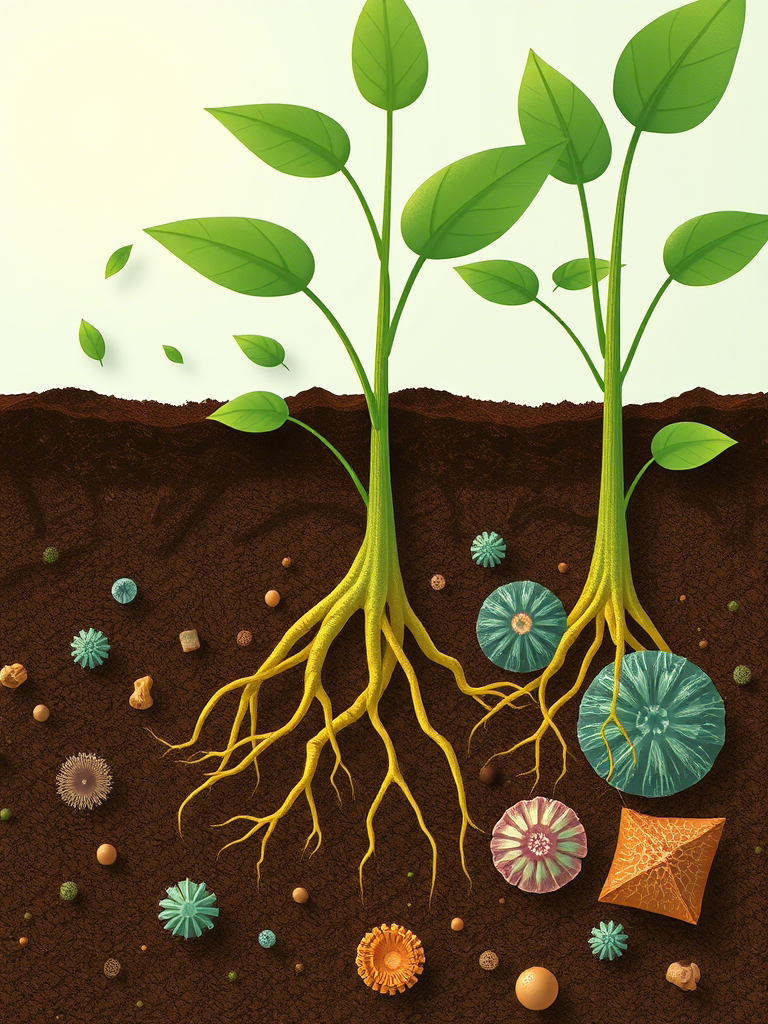
\includegraphics[width=\paperwidth,height=\paperheight]{figures/background.jpg}
%%}
%
%\begin{tikzpicture}[remember picture, overlay]
%
%% เพิ่มภาพพื้นหลังด้วยความโปร่งใส
%\node[opacity=0.5] at (current page.center) % ปรับความโปร่งใสที่นี่ (0.5 = 50%)
%{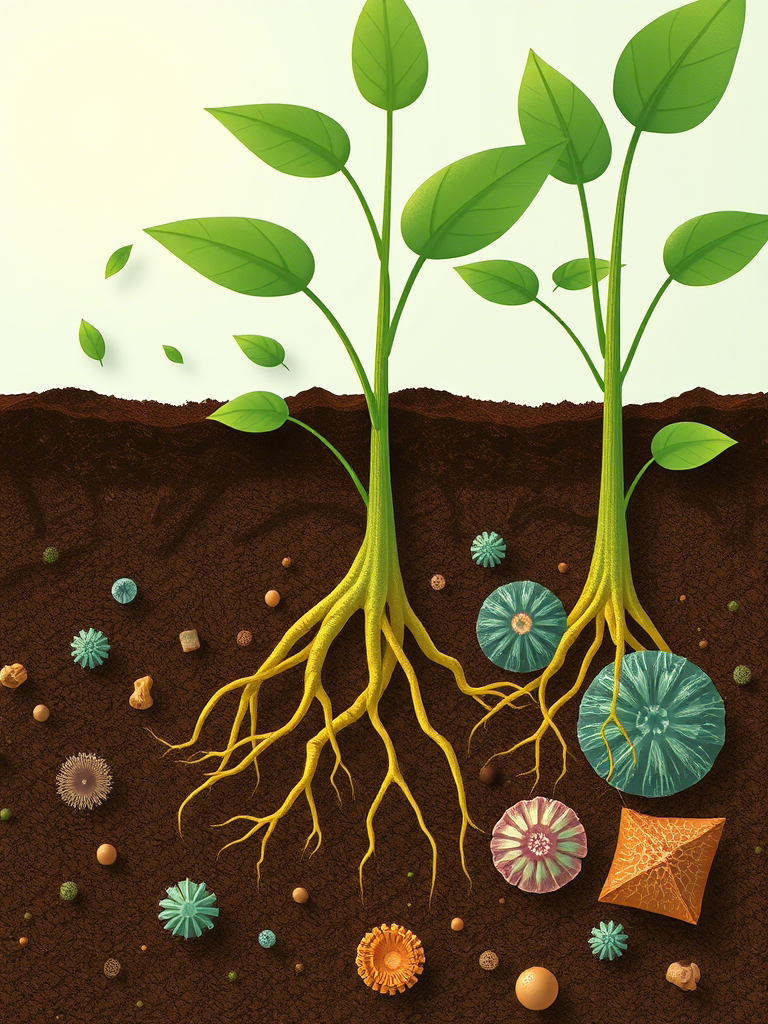
\includegraphics[width=\paperwidth,height=\paperheight]{figures/background.jpg}};
%
%
%% ใช้ tikzpicture เพื่อจัดตำแหน่งข้อความด้วยพิกัด (x, y)
%\begin{tikzpicture}[remember picture, overlay]
%
%% กล่องชื่อหนังสือ (เพิ่มความโปร่งแสง)
%\node[rectangle, draw=green!10, fill=green!10, opacity=0.8, rounded corners, minimum width=12cm, minimum height=3cm] 
%at ([yshift=10cm] current page.center)% จัดตำแหน่งกล่องที่กึ่งกลางหน้า
%{\fontsize{55}{28}\selectfont\color{orange} \textbf{จุลชีววิทยาเพื่อการเกษตร}};
%
%% ชื่อผู้แต่ง (จัดตำแหน่งด้วยพิกัด)
%\node[font=\fontsize{38}{22}\selectfont, text=white] 
%at ([yshift=-11cm] current page.center) % ปรับตำแหน่ง y ลงมา 5cm จากกึ่งกลาง
%{\textbf{จิรภัทร จันทมาลี}};
%
%% วันที่ (จัดตำแหน่งด้วยพิกัด)
%\node[font=\fontsize{34}{16}\selectfont, text=yellow] 
%at ([yshift=-13cm] current page.center) % ปรับตำแหน่ง y ลงมา 7cm จากกึ่งกลาง
%{\thaidate};
%
%\end{tikzpicture}
%
%
%\end{titlepage}
%\clearpage
%


\begin{titlepage}
\centering

% ใช้ tikzpicture เพื่อจัดตำแหน่งข้อความและภาพพื้นหลัง
\begin{tikzpicture}[remember picture, overlay]

% เพิ่มภาพพื้นหลังด้วยความโปร่งใส
\node[opacity=0.7] at (current page.center) % ปรับความโปร่งใสที่นี่ (0.5 = 50%)
{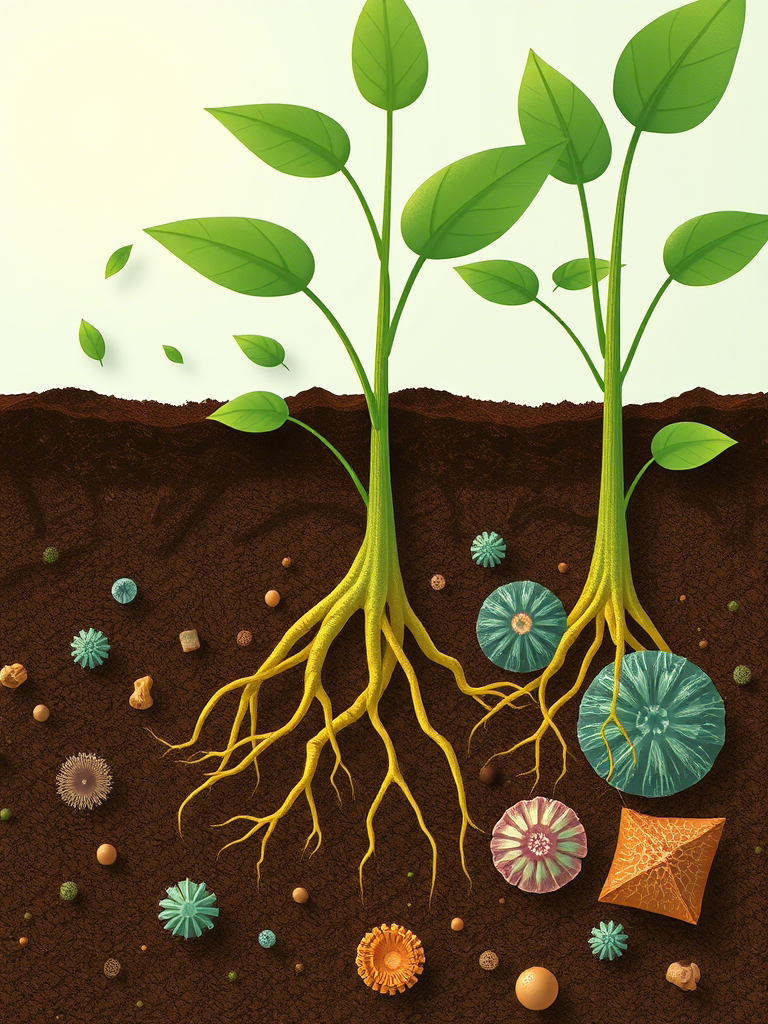
\includegraphics[width=\paperwidth,height=\paperheight]{figures/background.jpg}};

% กล่องชื่อหนังสือ (เพิ่มความโปร่งแสง)
\node[rectangle, draw=green!10, fill=green!10, opacity=0.7, rounded corners, minimum width=12cm, minimum height=3cm] 
at ([yshift=10cm] current page.center) % จัดตำแหน่งกล่องที่กึ่งกลางหน้า
{\fontsize{55}{28}\selectfont\color{orange} \textbf{จุลชีววิทยาเพื่อการเกษตร}};

% ชื่อผู้แต่ง (จัดตำแหน่งด้วยพิกัด)
\node[font=\fontsize{38}{22}\selectfont, text=white] 
at ([yshift=-11cm] current page.center) % ปรับตำแหน่ง y ลงมา 11cm จากกึ่งกลาง
{\textbf{จิรภัทร จันทมาลี}};

% วันที่ (จัดตำแหน่งด้วยพิกัด)
\node[font=\fontsize{34}{16}\selectfont, text=yellow] 
at ([yshift=-13cm] current page.center) % ปรับตำแหน่ง y ลงมา 13cm จากกึ่งกลาง
{\thaidate};

\end{tikzpicture}

\end{titlepage}
\clearpage
